\documentclass{tufte-handout}

\usepackage{ntheorem}
\usepackage{graphicx}
\usepackage{amsmath}
\usepackage{amssymb}
\usepackage{hyperref}
\usepackage{epigraph}
\theoremstyle{break}
% \usepackage[
% bibencoding=utf8,% .bib file encoding
% maxbibnames=3, % otherwise et al
% minbibnames=1, % otherwise et al
% backend=biber,%
% sortlocale=en_US,%
% style=apa,% or authoryear
% % apabackref=false, % backreferences
% natbib=true,% for citet/citep, but this is for backward compatibility
% uniquename=false,%
% url=true,%
% sortcites=false,
% doi=true,%
% eprint=true%
% ]{biblatex}
% \addbibresource{lecture_note_bib.bib}

\hypersetup{
  colorlinks,
  urlcolor = blue,
  pdfauthor={Paul Goldsmith-Pinkham}
  pdfkeywords={econometrics}
  pdftitle={Lecture Notes for Applied Empirical Methods}
  pdfpagemode=UseNone
}
\newtheorem{ruleN}{Rule}
\newtheorem{thmN}{Theorem}
\newtheorem{assN}{Assumption}
\newtheorem{defN}{Definition}
\newtheorem{exmp}{Example}
\newtheorem{cmt}{Comment}
\newtheorem{discussion}{Discussion Questions}
\newtheorem{proof}{Proof}

\newcommand{\continuation}{??}
\newtheorem*{excont}{Example \continuation}
\newenvironment{continueexample}[1]
 {\renewcommand{\continuation}{\ref{#1}}\excont[continued]}
 {\endexcont}
\newcommand{\bY}{\mathbf{Y}}
\newcommand{\bX}{\mathbf{X}}
\newcommand{\bD}{\mathbf{D}}
\newcommand{\E}{\mathbb{E}}

\newcommand\independent{\protect\mathpalette{\protect\independenT}{\perp}}
\def\independenT#1#2{\mathrel{\rlap{$#1#2$}\mkern2mu{#1#2}}}
\DeclareMathOperator{\Supp}{Supp}

\usepackage{cleveref}
\crefname{appsec}{appendix}{appendices}
\crefname{appsubsec}{appendix}{appendices}
\crefname{assumption}{assumption}{assumptions}
\crefname{equation}{equation}{equations}
\crefname{exmp}{example}{examples}
\crefname{assN}{assumption}{assumptions}
\crefname{cmt}{comment}{comments}
\crefname{defN}{definition}{definitions}

\usepackage[nolist]{acronym}
\begin{acronym}
  \acro{CI}{confidence interval}%
  \acro{OLS}{ordinary least squares}%
  \acro{CLT}{central limit theorem}%
  \acro{IV}{instrumental variables}%
  \acro{ATE}{average treatment effect}%
  \acro{RCT}{randomized control trial}%
  \acro{SUTVA}{stable unit treatment value assignment}
  \acro{VAM}{value-added model}%
  \acro{LAN}{locally asymptotically normal}%
  \acro{DiD}{difference-in-differences}%
  \acro{OVB}{omitted variables bias}
  \acro{FWL}{Frisch-Waugh-Lovell}
  \acro{DAG}{directed acyclic graph}
  \acro{PO}{potential outcomes}
\end{acronym}

\def\inprobHIGH{\,{\buildrel p \over \rightarrow}\,} 
\def\inprob{\,{\inprobHIGH}\,} 
\def\indistHIGH{\,{\buildrel d \over \rightarrow}\,} 
\def\indist{\,{\indistHIGH}\,}

\usepackage[many]{tcolorbox} 
\definecolor{main}{HTML}{5989cf}    % setting main color to be used
\definecolor{sub}{HTML}{cde4ff}     % setting sub color to be used
\definecolor{sub2}{HTML}{fde9ce}     % setting sub color to be used

\tcbset{
    sharp corners,
    colback = white,
    before skip = 0.2cm,    % add extra space before the box
    after skip = 0.5cm      % add extra space after the box
}                           % setting global options for tcolorbox

\newtcolorbox{boxD}{
    colback = sub, 
    colframe = main, 
    boxrule = 0pt, 
    toprule = 3pt, % top rule weight
    bottomrule = 3pt % bottom rule weight
}


\newtcolorbox{boxF}{
    colback = sub2,
    enhanced,
    boxrule = 1.5pt, 
    colframe = white, % making the base for dash line
    borderline = {1.5pt}{0pt}{main, dashed} % add "dashed" for dashed line
}

\newtcolorbox{boxK}{
    sharpish corners, % better drop shadow
    boxrule = 0pt,
    toprule = 4.5pt, % top rule weight
    enhanced,
    fuzzy shadow = {0pt}{-2pt}{-0.5pt}{0.5pt}{black!35} % {xshift}{yshift}{offset}{step}{options} 
}

\usepackage{tikz}
\usepackage{verbatim}
\usetikzlibrary{positioning}
\usetikzlibrary{snakes}
\usetikzlibrary{calc}
\usetikzlibrary{arrows}
\usetikzlibrary{decorations.markings}
\usetikzlibrary{shapes.misc}
\usetikzlibrary{matrix,shapes,arrows,fit,tikzmark}

\title{Lecture 1 - Potential Outcomes, Directed Acylic Graphs, and Structural Models}
\author{Paul Goldsmith-Pinkham}
\date{\today}


\begin{document}

\maketitle



Not every economics research paper is estimating a causal quantity. But, the implication or takeaway of papers is (almost) always a causal one.  Causality lies at the heart of every exercise. \sidenote{``We do not have knowledge of a thing until we have grasped its why, that is to say, its cause.'' -- Aristotle}

The goals in this lecture are:
\begin{itemize}
  \item Enumerate tools used to discuss causal questions
  \item Emphasize a \emph{multimodal} approach
  \item Set terminology/definitions for future discussions
\end{itemize}

Concretely, this involves covering three ways, notationally, of considering 
causal questions:
\begin{enumerate}
  \item the potential outcomes (PO) framework,
  \item the directed acyclic graph (DAG) framework,
  \item structural models. 
\end{enumerate}

Over the course of describing these, we will also refresh our memories on the difference between the estimator, the estimand and the estimate, and learn the identification condition for the average treatment effect (ATE).

\section{Notation}
We will begin by outlining some notation for potential outcomes. 
When defining treatment effects, this notation is extremely convenient and 
clear, particularly when considering settings with significant unobserved heterogeneity.
However, since so much of the extant literature in economics (and econometrics) is
written using more standard structural equations (e.g. $Y = X\beta + \epsilon$),
it is important to be able to translate between the two. For the sake of completeness,
I also want to expose you to the directed acyclic graph (DAG) framework, \citep{pearl2009causality, imbens2020potential} 
which is more commonly used in other fields such as epidimiology and computer science.\footnote{There was a period of time when the debate about DAGs was quite ornery (especially online). I think this has subsided.} It is 
much less common in economics, but without getting into broader epistemic debates, it's 
extremely useful in some settings for clarifying the identifying assumptions (especially in
settings relying on a ``conditional on observables'' assumption).

\section{Potential Outcomes}
We will follow \citet{imbens2015causal} in our notation. I will be slightly looser in my definitions for the purpose of space, but I encourage you to read Chapter 1 of \citet{imbens2015causal} or Chapter 7 of \citet{aronow2019foundations} for a more precise treatment.

Consider a sample of $N$ units, indexed by $i$. Each unit has a treatment status $D_i$ and an outcome $Y_i$.\footnote{For now, we will assume that there is just a binary treatment, but this can be generalized to multiple or continuous treatments. It will make life more complicated.} Sometimes, I will refer to the collection of observations or treatments as $\bD$ and $\bY$ to denote a vector of length $N$ with each element corresponding to the treatment or outcome for a given unit. Both $\bD$ and $\bY$ are \emph{observed} in our data: we see who is treated ($\bD$), and the subsequent outcome (the $\bY$ given the $\bD$)


\begin{boxD}
  \begin{exmp}
    \label{example1}
    Many medical examples naturally lend themselves to thinking about potential outcomes. For example, consider the outcome of whether you have a headache in three hours:
    \begin{equation*}
      Y = \begin{cases}
        1 & \; \text{Have a headache in three hours} \\
        0 & \; \text{Do not have a headache in three hours}
      \end{cases}
    \end{equation*}
    and the treatment of taking an aspirin:
    \begin{equation*}
      D = \begin{cases}
        1 & \; \text{Take an aspirin} \\
        0 & \; \text{Do not take an aspirin}.
      \end{cases}
    \end{equation*}
  \end{exmp}
  \end{boxD}

We now consider the \emph{potential} outcome for unit $i$. We can denote this as $Y_{i}(\bD)$, which is the outcome for unit $i$ if the set of treatments for the $N$ units is $\bD$. Note that this is a complicated function! It depends on the treatment status of all units, not just the treatment status of unit $i$. This leads us to a first important assumption:
\begin{assN}[Stable Unit Treatment Value Assumption]
  If $D_{i}$ = $D_{i}'$, then $Y_{i}(\bD) = Y_{i}(\bD')$.
\end{assN}
Put in words, it means that your potential outcome is only affected by your own treatment status, and not the treatment status of others.\footnote{Sometimes this is called a ``no interference'' condition. As we'll see later on, this could also be labeled a spillover in the economics literature.} This assumption lets us write our potential outcome as $Y_{i}(D_{i})$, and focus just on how our own treatment affects our outcome. This is a strong assumption; we will discuss how one might consider relaxing it in a few lectures. And of course any macroeconomist will tell you that this is a terrible assumption. But, it is a useful starting point. 


\begin{boxD}
\begin{continueexample}{example1}
  We can now consider the \emph{potential} outcome in the state of the world where a person takes an aspirin or not: $Y_{i}(1)$ vs. $Y_{i}(0)$. Note that it is not fundamentally possible to observe both states of the world: even if a person were observed in different time periods, and in one case they took the aspirin and in another they did not, this would reflect fundamentally different observations. This type of repeated observation could be used to help identify the average potential outcomes, but would require additional assumptions.


  SUTVA is a very natural assumption in our medical example, since others' aspirin treatment decision should have no impact on our headache. However, this is likely not true with vaccines or other interventions.
  \end{continueexample}
\end{boxD}

It's worth remarking on a few things. First, this potential outcome  is an  function of the individuals' treatment status, and allowed to vary by individual. Second, this outcome itself is not necessarily observed. Indeed, what we observe is 
\begin{equation}
  Y_{i} = Y_{i}(1)D_{i} + Y_{i}(0)(1-D_{i}).
\end{equation}
Hence, for the untreated units, we observe their $Y_{i}(0)$, and vice versa for the treated units. This model is often referred to as the Neyman-Rubin Causal model.\footnote{These were not coauthors - Jerzy Neyman was a Polish statistician who initially proposed the potential outcomes framework to study completely randomized experiments \citep{neyman1990}. This model was adopted and expanded by Donald Rubin in a number of influential papers. This model was coined the Rubin Causal model by Paul Holland, in an influential paper \citep{holland1986statistics} about statistics and causality that we will revisit shortly.}

The fact that we only observe either $Y_{i}(1)$ or $Y_{i}(0)$ is sometimes called the ``fundamental problem of causal inference.\footnote{This term, again, comes from \citet{holland1986statistics} (which you should read!).}'' Since we can only observe one outcome for a given unit, we cannot trace out the counterfactual outcomes for a single unit. This makes  it quite challenging to know what the effect of changing $D_{i}$ is on a single unit $i$.\footnote{If we assume the treatment effects everyone exactly the same, then it is straightforward. While we might make a homogeneity assumption like this, we don't always believe it in practice.} 

One way to view the fundamental problem of causal inference is as a missing data problem.\footnote{The treatment by \citet{aronow2019foundations} covers this in very nice detail.} We will use many different techniques throughout this course to impute a counterfactual outcome such that we can know the causal effect of an intervention. 


\begin{boxF}
  \begin{cmt}
    It is worth thinking a bit about what causal effect you are interested in estimating. Often this is referred to as the \textbf{estimand}. This could be many things:
    \begin{itemize}
      \item A structural parameter ($d\text{Investment}/d\text{TaxRate}$?)
      \item The effect of zoning restrictions on housing supply
      \item A policy evaluation of a renter's assistance program
      \item The existence of underreaction in stock prices to earnings news
    \end{itemize}
    \end{cmt}
  \end{boxF}


\begin{boxF}
  \begin{cmt}
    It is important to get these terms straight. 
    \begin{itemize}
  \item \underline{Estimand}: the quantity to be estimated
  \item \underline{Estimate}: the approximation of the estimand using a finite data sample
  \item \underline{Estimator}: the method or formula for arriving at the estimate for an estimand
    \end{itemize}
    For a particularly goofy way to remember this: \url{https://twitter.com/paulgp/status/1275135175966494721?s=20}
    \end{cmt}
  \end{boxF}

\section{Identification of the Average Treatment Effect Estimand}
We will conclude this lecture by describing sufficient conditions under which we can identify the \textbf{Average Treatment Effect} or ATE, a common target estimand for researchers. 

Before we do that, we need to define the individual level causal estimand (that is, recall, inherently unknowable). Call this the \textbf{Individual Treatment Effect} or ITE. This is the difference between the potential outcomes for a given unit:
\begin{equation}
  \tau_{i} \equiv Y_{i}(1) - Y_{i}(0). 
\end{equation}
This can be easily generalized to multiple treatments as well: we will discuss this in a few lectures.

\subsection{Average Treatment Effect}
We now consider the \emph{average} treatment effect over the population. This is, quite simply, the average of the individual treatment effects over all individuals in the overall population.
\begin{defN}
  We define the average treatment effect in our population as 
  \begin{equation*}
    \tau_{ATE} \equiv \E(\tau_{i}) = \E(Y_{i}(1) - Y_{i}(0)) = \E(Y_{i}(1)) - \E(Y_{i}(0)).
  \end{equation*}
\end{defN}

Why do we find the ATE interesting?\footnote{This is sometimes called the \emph{population average treatment effect} or PATE. This is then contrasted with the \emph{sample average treatment effect} or SATE. The SATE is the ATE defined for the sample of $N$ individuals we observe, while the PATE is the ATE for the population of individuals we can draw the sample from. We will discuss this in more detail later in the class, but for now I will just refer to the ATE to refer to the average treatment effect over the  sample, and assume that the SATE and PATE are similar. Typically if samples are randomly draw, this is a reasonable assumption, and the difference is mainly in the inference. See \citet{imbens2004nonparametric} for an example discussion. } For one thing, it describes the effect of giving the treatment to everyone in the population. This is often of interest to policymakers, who want to know the effect of a policy on the entire population.

We now consider some additional average treatment estimands. The first is the Average Treatment Effect on the Treated (ATT):
\begin{defN}
  \begin{equation*}
    \tau_{ATT} \equiv \E(\tau_{i}| D_{i} = 1) = \E(Y_{i}(1) | D_{i} = 1) - \E(Y_{i}(0)| D_{i} = 1).
  \end{equation*}
\end{defN}
This estimates the effect for individuals who received the treatment.\footnote{It will be a little while until we discuss cases when the ATT and ATE are different. A notable example is difference-in-differences. Many examples where we use \emph{models} to estimate our counterfactual outcome will lead to cases where we can only identify the ATT and not the ATE.} Note that one piece of the ATT is observed: $E(Y_{i}(1) | D_{i} = 1)$. This is just the observed outcome for the treated units. 

We can also define the conditional average treament effect (CATE). Let $X_{i}$ be a pre-determined set of covariates. Then, we can define the CATE as:
\begin{defN}
  \begin{equation*}
    \tau_{CATE}(x) \equiv \E(Y_{i}(1) | X_{i} = x) - \E(Y_{i}(0)| X_{i} = x).
  \end{equation*}
\end{defN}


\begin{boxD}
  \begin{continueexample}{example1}
    The ATE is what the effect would be on headaches if every person in the population took aspirin relative to not taking aspirin.

    The ATT is what the impact of aspirin has been for those who took aspirin, relative to if they had not taken aspirin.

    The CATE is what the impact of aspirin for a particular group, such as older men, would be relative to not taking aspirin.
    \end{continueexample}
  \end{boxD}

It is useful to note the following relationship between the ATE and the CATE:
\begin{equation*}
  \tau_{ATE} = \int \tau_{CATE}(x) f(x) dx.
\end{equation*}
If $X_{i}$ is discrete with values in $\mathcal{X}$, more simply this is
\begin{equation*}
  \tau_{ATE} = \sum_{x \in \mathcal{X}} \tau_{CATE}(x) Pr(X_{i} = x).
\end{equation*}

We now discuss under what conditions we can identify the ATE. 

\subsection{Identification of the ATE}

\begin{boxF}
  \begin{cmt}
    What is identification? Intuitively, for a given estimand to be identified, it means that in a world with no uncertainty about data, can we always identify the value of our estimand from the data we observe?

    To quote \citet{lewbel2019identification}: ``Econometric identification really means just one thing: model parameters or features being uniquely determined from the observable population that generates the data.''

%    As we will see later in the course, there is a bit of a tension in th
    \end{cmt}
  \end{boxF}

Note that without further assumptions, the ATE is not identified from the observed data, $(\bY, \bD)$. Why? Consider the following estimator of the ATE:

\begin{equation}
  \label{eq:ate_naive}
  \tau = E(Y_{i} | D_{i} = 1) - E(Y_{i} | D_{i} = 0)
\end{equation}
which compares the treated units' average outcome to the untreated units' average outcome. Rewriting using our potential outcomes,
\begin{equation*}
  \tau = E(Y_{i}(1) | D_{i} = 1) - E(Y_{i}(0) | D_{i} = 0),
\end{equation*}
we see that our key challenge is that the two expectations condition on \emph{different} values of $D_{i}$. Hence, if there is correlation between $D_{i}$ and $(Y_{i}(1), Y_{i}(0))$, these two averages are not comparable. 

\begin{boxD}
  \begin{exmp}
    \label{ex:example2}
    Imagine I am a researcher studying the effect of a wage training program ($D_{i}$) on wages ($Y_{i}$). I have a sample of workers, and I observe their wages and whether they participated in the training program. I want to know the effect of the training program on wages. If I use \Cref{eq:ate_naive} to compare the wages of those who take the program to those who do not, I may be comparing individuals who are very different. 
    \linebreak

    For example, if the training program is voluntary, then it is likely that those who take the program are more motivated or knowledgeable about the labor force, and hence would have higher wages even if they did not take the program. In this case, the naive estimator would overstate the effect of the training program on wages. Let $U_{i}$ be a binary variable capturing their motivation or knowledge of the labor force. If $E(D_{i} | U_{i} = 1) - E(D_{i} | U_{i} = 0)  > 0$, and $E(\tau_{i} | U_{i} = 1) - E(\tau_{i} | U_{i} = 0)  > 0$, then the naive estimator will overstate the effect of the training program on wages.
  \end{exmp}
\end{boxD}

\begin{boxF}
  \begin{cmt}
    As an exercise, prove that the naive estimator is biased in \Cref{ex:example2}.
    \end{cmt}
  \end{boxF}

We are now ready for our first identification result. We first define \textbf{strong ignorability}:
\begin{defN}
  \label{def:strong_ignorability}
  We say that $D_{i}$ is strongly ignorable conditional on a vector $\bX_{i}$ if
  \begin{enumerate}
\item     $Y_{i}(0), Y_{i}(1) \perp D_{i} | \bX_{i}$
\item $\exists \varepsilon > 0$ such that $\varepsilon < Pr(D_{i} = 1 | \bX_{i}) < 1-\varepsilon$.
  \end{enumerate}
\end{defN}
The first part of \Cref{def:strong_ignorability} is sometimes referred to unconfoundeness (or in economics, exogeneity): we assume that the choice of treatment is independent (conditional on $\bX$) of the units' potential outcome. This means a unit can't select into the treament based on their potential benefits.\footnote{Strong ignorability is a much more precise term than exogeneous, but tends to be used less in economics. When communicating with an economics audience, you might say that $D_{i}$ is conditionally randomly assigned, or $D_{i}$ is exogeneous -- but this would omit the second condition (which is that the treatment is not too rare or too common).}

The second condition asserts that there is some variation in treatment. This is sometimes called the common support or overlap condition . It is a bit stronger than we need, but it is a convenient way to ensure that we can compare the treated and untreated units.

\begin{thmN}[Identification of the ATE]
  \label{thm:ate_identification}
If $D_{i}$ is strongly ignorable conditional on $\mathbf{X}_{i}$, then
  \begin{equation*}
    \mathbb{E}(\tau_{i}) = \sum_{x \in \Supp X_{i}} \bigg(\mathbb{E}(Y_{i} | D_{i} = 1, \mathbf{X}_{i} = x) - \mathbb{E}(Y_{i} | D_{i} = 0, \mathbf{X}_{i} = x)\bigg)Pr(\mathbf{X}_{i} = x)
  \end{equation*}
\end{thmN}
\begin{proof}
  Note that by strong ignorability,
  \begin{equation*}
    \mathbb{E}(Y_{i}(0) | \mathbf{X}_{i} ) = \mathbb{E}(Y_{i}(0) | D_{i} = 0, \mathbf{X}_{i} ) = \mathbb{E}(Y_{i}
  | D_{i} = 0, \mathbf{X}_{i}).
  \end{equation*} 
  In essence,
  independence of $D_{i}$ and $(Y_{i}(0), Y_{i}(1))$ lets us
  interchange counterfactuals and realized data in conditionals. The
  rest follows by the law of iterated expectations. 
\end{proof}

This result is quite powerful, and describes a non-parametric condition for when we can identify (and estimate) the ATE. A corrolary of this theorem is that we can also identify conditional average treatment effects as well (by assumption).

\section{Identification through Directed Acylic Graphs}

Above, we encoded random variables' relationships functionally, using potential outcomes. An alternative approach does this graphically. I will not cover this in significant detail, but want to give an example of how to think about identification using Directed Acylcic Graphs (DAGs). 

 We can encode the relationship between $D$ and $Y$ using an \emph{arrow} in a graph. The direction emphasizes that $D$ causes $Y$, and not vice versa.  
 
 \begin{figure}
  \begin{center}
  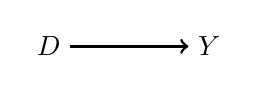
\begin{tikzpicture}
        \node[text centered] (t) {$D$};
        \node[right=1.5 of t, text centered] (y) {$Y$};
        \draw [->, line width= 1] (t) -- (y);
   \end{tikzpicture}
   \caption{$D$ has a causal effect on $Y$}
  \end{center}
  \end{figure}

  We can also allow for the unobservable $U$, which drove
  identification concerns above in \Cref{ex:example2}. In this case, $U$ is termed a \emph{confounder}. We can look at the paths by which $D$ links to $Y$:
  \begin{itemize}
  \item The standard direct effect $D \rightarrow Y$
  \item The ``back door'' path $D \leftarrow U \rightarrow Y$
  \end{itemize}
 Note that the back-door is \emph{not} causal. We know from above that the effect of $D$ on $Y$ is not identified under this setup, but this provides a graphical intuition as well -- there is a path connecting $D$ and $Y$ but it does not flow in the right direction.

 \begin{figure}
\begin{center}
  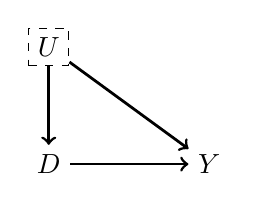
\begin{tikzpicture}
    % nodes %
    % \node[text centered] (z) {$Z$};
    \node[text centered] (t) {$D$};
    \node[right=1.5 of t, text centered] (y) {$Y$};
    \node[draw, rectangle, dashed, above = 1 of t, text centered] (u) {$U$};

    % edges %
    % \draw[->, line width= 1] (z) --  (t);
    \draw [->, line width= 1] (t) -- (y);
    % \draw[->,red, line width= 1,dashed] (u) --node {X} (z);
    \draw[->,line width= 1] (u) --(t);
    \draw[->,line width= 1] (u) -- (y);
%\draw[->, red, line width=1,dashed] (z) to  [out=270,in=270, looseness=0.5] node{X} (y);
  \end{tikzpicture}
\end{center}
\caption{$D$'s effect on $Y$ is confounded by $U$}
\end{figure}

Now, we can replace $U$ with an observable $X$.  $X$ is still a confounder, but since it is observable, we can condition on it and identify our effect (as in \ref{thm:ate_identification}). As before, examine the paths by which $D$ links to $Y$:
\begin{itemize}
\item The standard direct effect $D \rightarrow Y$
\item The ``back door'' path $D \leftarrow X \rightarrow Y$.
\end{itemize}

In a DAG, conditioning on a variable along the path
``blocks'' the path, such that we would block the back door path. 

\begin{figure}
\begin{center}
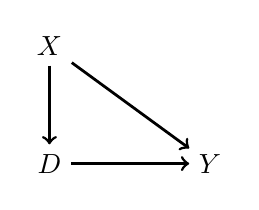
\begin{tikzpicture}
  % nodes %
  % \node[text centered] (z) {$Z$};
  \node[text centered] (t) {$D$};
  \node[right=1.5 of t, text centered] (y) {$Y$};
  \node[above = 1 of t, text centered] (u) {$X$};

  % edges %
  % \draw[->, line width= 1] (z) --  (t);
  \draw [->, line width= 1] (t) -- (y);
  % \draw[->,red, line width= 1,dashed] (u) --node {X} (z);
  \draw[->,line width= 1] (u) --(t);
  \draw[->,line width= 1] (u) -- (y);
%\draw[->, red, line width=1,dashed] (z) to  [out=270,in=270, looseness=0.5] node{X} (y);
\end{tikzpicture}
\end{center}
\caption{$D$'s effect on $Y$ is confounded by an observable $X$}
\end{figure}

Finally, let's consider a more complicated example. $X$ is now a ``collider'', such that $D$ and $Y$ both affect $X$. 

\begin{figure}
  \begin{center}
    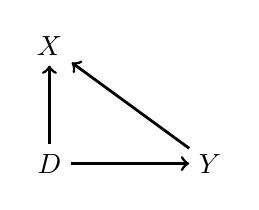
\begin{tikzpicture}
      % nodes %
      % \node[text centered] (z) {$Z$};
      \node[text centered] (t) {$D$};
      \node[right=1.5 of t, text centered] (y) {$Y$};
      \node[above = 1 of t, text centered] (u) {$X$};

      % edges %
      % \draw[->, line width= 1] (z) --  (t);
      \draw [->, line width= 1] (t) -- (y);
      % \draw[->,red, line width= 1,dashed] (u) --node {X} (z);
      \draw[<-,line width= 1] (u) --(t);
      \draw[<-,line width= 1] (u) -- (y);
%\draw[->, red, line width=1,dashed] (z) to  [out=270,in=270, looseness=0.5] node{X} (y);
    \end{tikzpicture}
  \end{center}
\end{figure}

As before, examine the paths by which $D$ links to $Y$:
    \begin{itemize}
    \item The standard direct effect $D \rightarrow Y$
    \item The indirect path $D \rightarrow X \leftarrow Y$.
    \end{itemize}
This is not called a backdoor path because $X$ does not point into $D$.  

The key difference in this setting is that since $X$ does not cause $Y$, it is automatically blocked (all effects on $X$ occur through our main effect). However, if you condition on $X$, you open the path! 

\begin{boxD}
\begin{continueexample}{ex:example2}
  Return to the example of a job training program. We want to study the impact of the program on wages, and we condition on whether a person has a car. If a person's wages affects their likelihood of having a car, we will have created a biased comparison: we will first consider the effect of the job training program among those who have a car (which may be small), and then among those who do not (which may also be small). If much of the effect of the program affects individuals' ability to buy a car, then we will underestimate the effect of the program.
\end{continueexample}
\end{boxD}
 
\begin{boxF}
  \begin{cmt}
    A last example is what's called a \emph{mediator}. This is another variable that is affected by the treatment, and affects the outcome. In this case, we can think of the treatment as having two effects: a direct effect, and an indirect effect through the mediator. 

    \centering  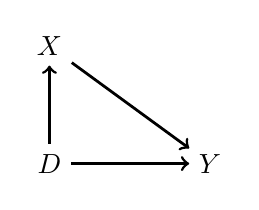
\begin{tikzpicture}
      % nodes %
      % \node[text centered] (z) {$Z$};
      \node[text centered] (t) {$D$};
      \node[right=1.5 of t, text centered] (y) {$Y$};
      \node[above = 1 of t, text centered] (u) {$X$};

      % edges %
      % \draw[->, line width= 1] (z) --  (t);
      \draw [->, line width= 1] (t) -- (y);
      % \draw[->,red, line width= 1,dashed] (u) --node {X} (z);
      \draw[<-,line width= 1] (u) --(t);
      \draw[->,line width= 1] (u) -- (y);
%\draw[->, red, line width=1,dashed] (z) to  [out=270,in=270, looseness=0.5] node{X} (y);
    \end{tikzpicture}

\raggedright
    It is possible to control for a mediator in order to estimate only the direct effect -- this is sometimes referred to as mediation analysis. However this is \emph{very} sensitive to functional form, and not recommended.
  \end{cmt}
\end{boxF}

I will not give an exhaustive approach on how to deal with DAGs for identification, but you can hopefully see that there is a great deal of intuitive value in writing down the DAG in some problems. This is particularly true when dealing with \emph{colliders}. 

\section{Structural equations and causal effects}
It is important to not lose sight of the fact that these should be estimates that inform our \emph{economic} model. Since much of our background is traditionally in structural equations (that often map to economic models) it can often be more familiar to write out outcome equation as:

\begin{equation*}
  Y_{i} = \alpha + \beta D_{i} + \varepsilon_{i}.
\end{equation*}

It is quite helpful to see how this maps back to the potential outcome framework:

\begin{align*}
  Y_{i} &= Y_{i}(0)(1 - D_{i}) + Y_{i}(1)D_{i}\\
  &= Y_{i}(0) + \tau_{i}D_{i}\\
  &= Y_{i}(0) + \tau D_{i} + (\tau_{i} - \tau)D_{i}\\
  &= \underbrace{E(Y_{i}(0) | D_{i} = 0)}_{\alpha} + \underbrace{\tau}_{\beta} D_{i} + \underbrace{(\tau_{i} - \tau)D_{i} + (Y_{i}(0)-E(Y_{i}(0) | D_{i} = 0))}_{\varepsilon_{i}}
\end{align*}

Consider now what $E(Y_{i} | D_{i})$ will recover:
\begin{align*}
  E(Y_{i} | D_{i} = 1) &= \alpha + \tau + E(\varepsilon_{i} | D_{i} = 1)\\
  E(\varepsilon_{i} | D_{i} = 1) &= (E(\tau_{i} | D_{i}=1) - \tau)  + E(Y_{i}(0) | D_{i} = 1) -  E(Y_{i}(0) | D_{i} = 0)\\
  E(Y_{i} | D_{i} = 0) &= \alpha + E(\varepsilon_{i} | D_{i} = 0)\\
  E(\varepsilon_{i} | D_{i} = 0) &= 0.
\end{align*}
So, we can see that we will recover the average treatment effect as $\beta$ if $D_{i}$ is randomly assigned (or strongly ignorable).  This is a special case where the coefficient $\beta$ in the linear regression case will give the average treatment effect, the constant will give the average for the untreated, and the error term will capture the rest. We will suffer from omitted variable bias if $ E(Y_{i}(0) | D_{i} = 1) -  E(Y_{i}(0) | D_{i} = 0) \neq 0$ -- e.g. if there is selection into treatment based on your control potential outcome. Notice that if $E(\tau_{i} | D_{i} =1) \not=\tau$, then we will also not estimate the ATE, but we will estimate the ATT.

%An interesting thing to notice is that under heterogeneity, this regression must have heteroskedasticity. 

More generally, however, it's just useful to see that there are one-to-one mappings between the potential outcome framework and structural regressions. In many ways, the potential outcome framework is helpful because it emphasizes the relevant counterfactual state more than many linear models. 

Phil Haile has \href{https://www.princeton.edu/~reddings/tradephd/Haile_theorymeas.pdf}{some lovely slides} discussing the importance of structure in economics. One of the key issues he pushes back on is the idea where many applied researchers estimating treatment effects say they are being ``model-free.'' In other words, rather than writing down a structural model and attempting to estimate something complicated with a functional form, they view their treatment effects as model-agnostic. This is sometimes referred to as the ``reduced form''.

What is the reduced form from a structural estimation perspective? Following Haile, a reduced form relationship is one where the endogeneous variable is a function of \emph{exogeneous} variables and unobserved structural error terms. Exogeneous here means variables that satisfy the necessary independence assumptions with the structural error terms.



\begin{boxD}
  \begin{exmp}
Consider a supply and demand system:
\begin{align*}
  Q_{d} &= D(P, X, U_{d})\\
  Q_{s} &= S(P, Z, U_{s}).
\end{align*}
These are simultaneous equations where the observed price we see in the market is the price where $Q_{d} = Q_{s}$. 
Often, supply ($Q_{s}$) will be written in terms of price (which is a function of marginal cost):
\begin{align*}
  Q &= D(P, X, U_{d})\\
  P &= S(Q, Z, U_{s}).
\end{align*}
Since $P$ and $Q$ are endogeneous, these are \emph{structural} equations. 
\linebreak

The reduced form version of these equations would have the form
\begin{align*}
  Q &= d(X, Z, U_{d}, U_{s})\\
 P &= s(X, Z, U_{d}, U_{s}).
\end{align*}

In economics, we may consider estimating the effect of price on quantity (e.g. a labor demand elasticity), which is a parameter in the structural demand equation. When we use instrumental variables and two-stage least squares (to be discussed further in a later class), the \emph{first stage} will be the reduce form, and the second stage is a structural model.
  \end{exmp}
  \end{boxD}

Overall, it's important to remember that many of our estimation approaches imply a particular structural model. We may be approximating something more complicated, but we're typically making some kind of modeling decision.

\begin{boxK}
  \begin{discussion}
    \begin{enumerate}
      \item Consider the potential outcome framework in the context of individuals. We are thinking about annual earnings $Y_{i}$ for an individual $i$. 
      Often, we study the earnings gap between men and women. Is it reasonable to consider the potential outcome $Y_{i}(1)$ vs. $Y_{i}(0)$ for $D_{i} =1$ when $i$ is a woman vs. when $i$ is a man?
      \item Consider the linear model  from above:
      \begin{equation*}
  Y_{i} = \alpha + \beta D_{i} + \varepsilon_{i}.
      \end{equation*}
      When would we expected homoskedasticity to hold? 
    \end{enumerate}
  \end{discussion}
\end{boxK}


\bibliography{lecture_note_bib.bib}
\bibliographystyle{plainnat}


\end{document}